\documentclass{../../oss-handout}
\usepackage{enumitem}
\usepackage{tikz}
\usepackage{siunitx}
\usepackage{newtxtext,newtxmath}
\usepackage{bm}

\sisetup{
  inter-unit-product=\cdot,
  per-mode=symbol
}
\tikzset{>=latex}

\setlength{\parindent}{0pt}
\setlength{\parskip}{6pt}
\setlength{\headheight}{26pt}

\newcommand{\pic}[2]{\includegraphics[width=#1\textwidth]{#2}}

% Set the page style for the document
\pagestyle{plain}

% Course & handout information
\renewcommand{\institution}{Olympiads School, Toronto, Ontario, Canada}
\renewcommand{\coursetitle}{AP Physics 1}
\renewcommand{\term}{Winter 2021}
\title{Solutions to Mock Exam \#1}
\author{Dr.\ Timothy Leung}
\date{\today}

\begin{document}
\thispagestyle{title}
\gentitle

\begin{enumerate}[leftmargin=15pt]
\item\textbf{(D)} For any projectile, there are two angles that have the same
  range, and the sum of the angle is \ang{90}. If one of the angle is \ang{60},
  then the other angle is \ang{30}.

\item\textbf{(B)} The maximum range occurs at \ang{45}, so the horizontal
  distance will \textbf{increase}.

\item\textbf{(C)} The driver of the car is rounding a circular path, so the
  centripetal force on the driver is provided by the difference between gravity
  (which contributes to $F_c$), and normal force (which contributes against
  $F_c$, and is what we are solving here), i.e.:
  \begin{align*}
    F_c &= F_g - F_N\\
    F_N &= F_g - F_c= mg- \frac{mv^2}{r}=m\left( g- \frac{v^2}{r}\right)=
    50\left(10-\frac{20^2}{50}\right)=50(10-8)=\boxed{\SI{100}{\newton}}
  \end{align*}

\item\textbf{(A)} The forces that $X$ and $Y$ exert on each other must be equal
  by the third law of motion, therefore
  \begin{equation*}
    \boxed{F_\text{up}=F_\text{down}}
  \end{equation*}
  When Block $Y$ is stationary, the acceleration is at its maximum, therefore
  the forces $F_\text{up}$ must be higher than the weight of block $Y$, $m_Yg$:
  \begin{equation*}
    \boxed{F_\text{up}>m_Yg}
  \end{equation*}
  
\item\textbf{(C)} There is no external net force, so when the water is added to
  the cart, the \textbf{total momentum is conserved}. As the mass increases, it
  means that the \textbf{velocity must decrease}.

\item\textbf{(D)}

\item\textbf{(B)} In a vacuum, both objects will have the same acceleration
  (due to gravity). If both are \emph{released} (i.e.\ dropped with zero
  initial velocity), then both will have the same \fbox{speed}.

\item\textbf{(B)} The ``block-Earth'' system does not include the spring, and
  so energy is conserved from B to C. If this is a ``spring-block-Earth''
  system, then the answer would be A.

\item\textbf{(B)} The reflected wave is in the same medium, and so it must have
  the same speed and amplitude as before (I and II are incorrect). It is
  reflected from a fixed end, and therefore the wave would be inverted (III).

\item\textbf{(B)} The area under both graphs are the same, and therefore the
  impulse is the same, which means that the change in momentum is the same.

\item\textbf{(A)} The definition of equilibrium is that an object is not
  subjected to any net external force.

\item\textbf{(C)} By the conservation of energy,
  \begin{align*}
    U_g &= K'+U_g'\\
    mgH &= \frac12mv^2+mgh'\\
    H &= \frac{v^2}{2g}+h'=\frac{3.0^2}{2\cdot9.8}+0.4=\boxed{\SI{.86}{\metre}}
  \end{align*}
  The calculation would have been \SI{.85}{\metre} if you used
  $g=\SI{10}{\metre\per\second\squared}$.

\item\textbf{(A)} The path that the block travels is curved, so at the bottom,
  there will be a centripetal force. In order to generate this centripetal
  force, \fbox{normal force $F_n$ must be greater than gravity $F_g$}.

\item\textbf{(C)} After the block leaves the track, it will travel as a
  projectile. The horizontal velocity is constant in a projectile, which we
  can calculate from when the block leaves the ramp. At the highest point of
  this projectile motion, it has the only horizontal component:
  \begin{displaymath}
    v_x=v\cos\ang{30}=3.0\cdot\cos\ang{30}=
    \boxed{\SI{2.6}{\metre\per\second}}
  \end{displaymath}

\item\textbf{(A)} Satellite 1 is closer to Earth than Satellite 2, therefore
  $F_1>F_2$, since gravitational force is inversely proportional to the square
  of the distance. We can obtain the orbital velocity by equating the
  centripetal force to gravitational force:
  \begin{equation*}
    F_c=F_g\quad\rightarrow\quad
    \frac{mv^2}{r}=\frac{GMm}{r^2}\quad\rightarrow\quad
    v=\sqrt{\frac{GM}{r}}
  \end{equation*}
  Satellite 1 is closer to Earth than Satellite 2, therefore it also has a
  higher speed.
  
\item\textbf{(D)} Work is positive if force is in the same direction as motion,
  and negative when it's opposite. It does not matter if the speed is constant
  or not.

\item\textbf{(D)} This is a completely inelastic collision because the carts
  stick together. Using conservation of momentum:
  \begin{displaymath}
    mv_i=(M+m)v_f \quad\rightarrow\quad
    v_f=\underbrace{\left(\frac{m}{M+m}\right)}_{\text{slope}}v_i
  \end{displaymath}
  
\item\textbf{(C)} A standing wave would like this. The nodes are located at
  $x=1,2,3$. The distance between nodes are half of the wavelength.
  \begin{center}
    \begin{tikzpicture}[xscale=1.7]
      \draw[very thick,->](0,0)--(3.3,0)    node[right]{$x$};
      \draw[very thick,->](0,-1.5)--(0,1.8) node[above]{$A$};
      \foreach \x in {.5,1.5,2.5} \draw(\x,.1)--(\x,-.1);
      \foreach \x in {1,2,3} \draw(\x,.1)--(\x,-.1) node[below]{\x};
      \draw[thick](0, 1.2)--(-.1, 1.2) node[left]{$0.003$};
      \draw[thick](0,-1.2)--(-.1,-1.2) node[left]{$-0.003$};
      \foreach \A in {-1.25,-1,...,1.25}{
        \draw[thick,smooth,samples=80,domain=0:3]
        plot({\x},{\A*sin(180*\x)});
      }
      \draw[|<->|,thick](.5,-1.5)--(2.5,-1.5) node[midway,below]{$\lambda$};
    \end{tikzpicture}
  \end{center}
  
\item\textbf{(D)} At equilibrium, the gravitational and spring forces on the
  \SI{3}{\kilo\gram} mass must balance, i.e.:
  \begin{equation*}
    mg=kx\quad\rightarrow\quad x=\left(\frac gk\right) m
  \end{equation*}
  The stretching of the spring at equilibrium is proportional to the mass $m$.
  Replacing the \SI3{\kilo\gram} mass with a \SI4{\kilo\gram} mass will
  increase the equilibrium stetch to $12\times\frac43=\SI{16}{\centi\metre}$
  which is also the magnitude of the ``oscillation'', if it happens. However,
  position when direction of motion is reversed is twice the amplitude, i.e.\
  $\boxed{\SI{32}{\centi\metre}}$.
  %\begin{center}
  %  \begin{tikzpicture}[xscale=1.7]
  %    \draw[very thick,->](0,0)--(3.3,0)    node[right]{$t$};
  %    \draw[very thick,->](0,-1.5)--(0,1.8) node[above]{$A$};
  %    \foreach \x in {.5,1.5,2.5} \draw(\x,.1)--(\x,-.1);
  %    \foreach \x in {1,2,3} \draw(\x,.1)--(\x,-.1) node[below]{\x};
  %    \draw[thick](0, 1.2)--(-.1, 1.2) node[left]{$A$};
  %    \draw[thick](0,-1.2)--(-.1,-1.2) node[left]{$-A$};
  %    \draw[very thick,smooth,samples=80,domain=0:2.6]
  %    plot({\x},{1.25*sin(180*\x)});
  %    \draw[|<->|,thick](.5,-1.5)--(2.5,-1.5) node[midway,below]{$\lambda$};
  %  \end{tikzpicture}
  %\end{center}
  
\item\textbf{(D)} As the wave moves, energy is dissipated by friction, therefore
  the amplitude decreases.

\item\textbf{(A)} The torque generated by the force is
  \begin{displaymath}
    \tau=FL\sin\theta
  \end{displaymath}
  If the force is applied perpendicularly, that would mean a moment arm of
  $\boxed{L\sin\theta}$.

\item\textbf{(D)} The total momentum of the third piece must cancel the momentum
  of the other two masses, i.e.:
  \begin{center}
    \begin{tikzpicture}
      \draw[->](0,0)--(-2,0) node[left]{$mV$};
      \draw[->](0,0)--(0,-2) node[right]{$mV$};
      \draw[ultra thick,->](0,0)--(-2,-2) node[left]{$\bm{p}=\sqrt2mV$};
    \end{tikzpicture}
  \end{center}
  The mass of the third piece is $3m$, therefore the velocity must be
  \begin{equation*}
    \bm{v}=\frac{\bm{p}}m
    =\frac{\sqrt2mV}{3m}=\boxed{\frac{\sqrt2}3V\;[\swarrow]}
  \end{equation*}
\item\textbf{(C)} Binrging the disk up to a higher angular velocity in the same
  time interval means a higher angular acceleration, which requires a higher
  torque $\tau=I\alpha$.
  \newpage
  
\item\textbf{(C)} The axle is horizontal, which means that the wheel rotates
  vertically. The torques genrated by the masses are drawn on the diagram:
  \begin{center}
    \begin{tikzpicture}[scale=2]
      \begin{scope}[thick]
        \draw(0,0) circle(1);
        \draw(-1,0)--(1,0);
        \draw[fill=gray](-1,0) circle(.05) node[left]{$m$};
        \draw[fill=gray]( 1,0) circle(.05) node[right]{$2M$};
        \draw[rotate=60](-1,0)--(1,0);
        \begin{scope}[rotate=-60]
          \draw (-1,0)--(1,0);
          \draw[fill=gray](-1,0) circle(.05) node[above left]{$M$};
          \draw[rotate around={60:(-1,0)},ultra thick,red,->] (-1,0)--(-1,-.5)
          node[below]{$\tau=MgR\sin\ang{30}$};
        \end{scope}
        \draw[fill=white](0,0) circle(.06);
      \end{scope}
      \draw[ultra thick,red,->] (1,0)--(1,-1) node[below]{$\tau=2MgR$};
      \draw[ultra thick,red,->] (-1,0)--(-1,-.7) node[below]{$\tau=mgR$};
    \end{tikzpicture}
  \end{center}
  If the wheel is in equilibrium, then the torques acting on it must sum to
  zero, i.e.
  \begin{displaymath}
    2MgR=mgR+\frac12MgR \quad\longrightarrow\quad\boxed{M=\frac23m}
  \end{displaymath}

\item\textbf{(E)} The angular momentum of an object is defined as:
  \begin{displaymath}
    L=rmv=4\cdot2\cdot 4.5=\boxed{\SI{24}{\kilo\gram\metre\per\second}}
  \end{displaymath}
   
\item\textbf{(D)} The weight of the beam acts at the center of mass, and
  generates a torque of
  \begin{displaymath}
    \tau_g=mg\frac{L}2=10\cdot9.8\cdot\frac22=\SI{98}{\newton\metre}
    \text{ [clockwise]}
  \end{displaymath}
  while the applied force generates a torque of
  \begin{displaymath}
    \tau_F=FL\sin\theta=200\cdot2\sin\ang{30}=\SI{200}{\newton.\metre}
    \text{ [counterclockwise]}
  \end{displaymath}
  The net torque is $\boxed{\tau_\text{net}=\SI{102}{\newton.\metre}}$
  counterclockwise.

\item\textbf{(C)} The maximum velocity of a spring-mass system is given by
  $v_\text{max}=A\omega$. The angular frequency is based on mass and spring
  constant. However, we still need the amplitude, which can be found from the
  maximum acceleration, $a_\text{max}=A\omega^2$, or $A=a_\text{max}/\omega^2$.

\item\textbf{(B)} The functions for velocity and acceleration is out of phase
  by \ang{90}.
  
\item\textbf{(A)} When Disk B is dropped onto Disk A, there is no external
  torque applied, therefore angular momentum remains the same. This means that
  the angular frequency $\omega$ is decreased by $\dfrac12$. The new kinetic
  energy is therefore
  \begin{displaymath}
    K'=\frac12I'\omega'^2=\frac12\cdot2I\cdot\left(\frac{\omega}2\right)^2
    =\frac12K
  \end{displaymath}
  And the kinetic energy is decreased to $\dfrac12$ of its original value.
\end{enumerate}
\end{document}
